\section{Geometric deep learning}

GDL (\textit{\textbf{G}eometric \textbf{D}eep \textbf{L}earning}) is involved with modeling neural
networks that satisfy invariances by design. Assume we have a set of feature vectors $\{ \vec{x}_1,
    \ldots, \vec{x}_M \} \subset R$ over which we want to realize a function $f: \mathcal{P}(R) \to
    \mathcal{Y}$. Naively, we could concatenate the set into a single feature vector and apply a
standard multi-layer perceptron, \[
    \{ \vec{x}_1, \ldots, \vec{x}_M \} \mapsto [\vec{x}_1, \ldots, \vec{x}_M].
\]
However, this has two problems---(1) $M$ is not fixed, so the inputs have variable length and (2)
the order in which we concatenate the feature vectors is arbitrary. We need to model an
architecture that can take a variable-length input and does not depend on the ordering of the
feature vectors.

\subsection{Invariance and equivariance in neural networks}

In order to formally design such functions, we need the following two definitions.

\begin{definition}[Order-invariance]
    $f: \mathcal{P}(R) \to \mathcal{Y}$ is order-invariant if and only if \[
        f(\vec{x}_1, \ldots, \vec{x}_M) = f(\vec{x}_{\pi_1}, \ldots, \vec{x}_{\pi_M}), \quad \forall \vec{\pi} \in \Pi(M),
    \]
    where $\vec{\pi}$ is a permutation. Or, in matrix notation, \[
        f(\mat{X}) = f(\mat{P} \mat{X}),
    \]
    where $\mat{X} \in \R^{M\times d}$ contains the feature vectors and $\mat{P} \in \R^{M \times M}$
    is a permutation matrix.
\end{definition}

\begin{definition}[Equivariance]
    $f: R^M \to \mathcal{Y}^M$ is equivariant if and only if
    \begin{align*}
        f(\vec{x}_1, \ldots, \vec{x}_M)                      & = (y_1, \ldots, y_M)                                                  \\
        \implies f(\vec{x}_{\pi_1}, \ldots, \vec{x}_{\pi_M}) & = (y_{\pi_1}, \ldots, y_{\pi_M}), \quad \forall \vec{\pi} \in \Pi(M).
    \end{align*}
    Or, in matrix notation, \[
        f(\mat{X}) = \mat{P} f(\mat{P}\mat{X}),
    \]
    where $\mat{X} \in \R^{M\times d}$ contains the feature vectors and $\mat{P} \in \R^{M\times M}$ is
    a permutation matrix.
\end{definition}

The question thus becomes how we can design model architectures that are order-invariant or
equivariant.

\subsection{Deep sets}

\begin{figure}[t]
    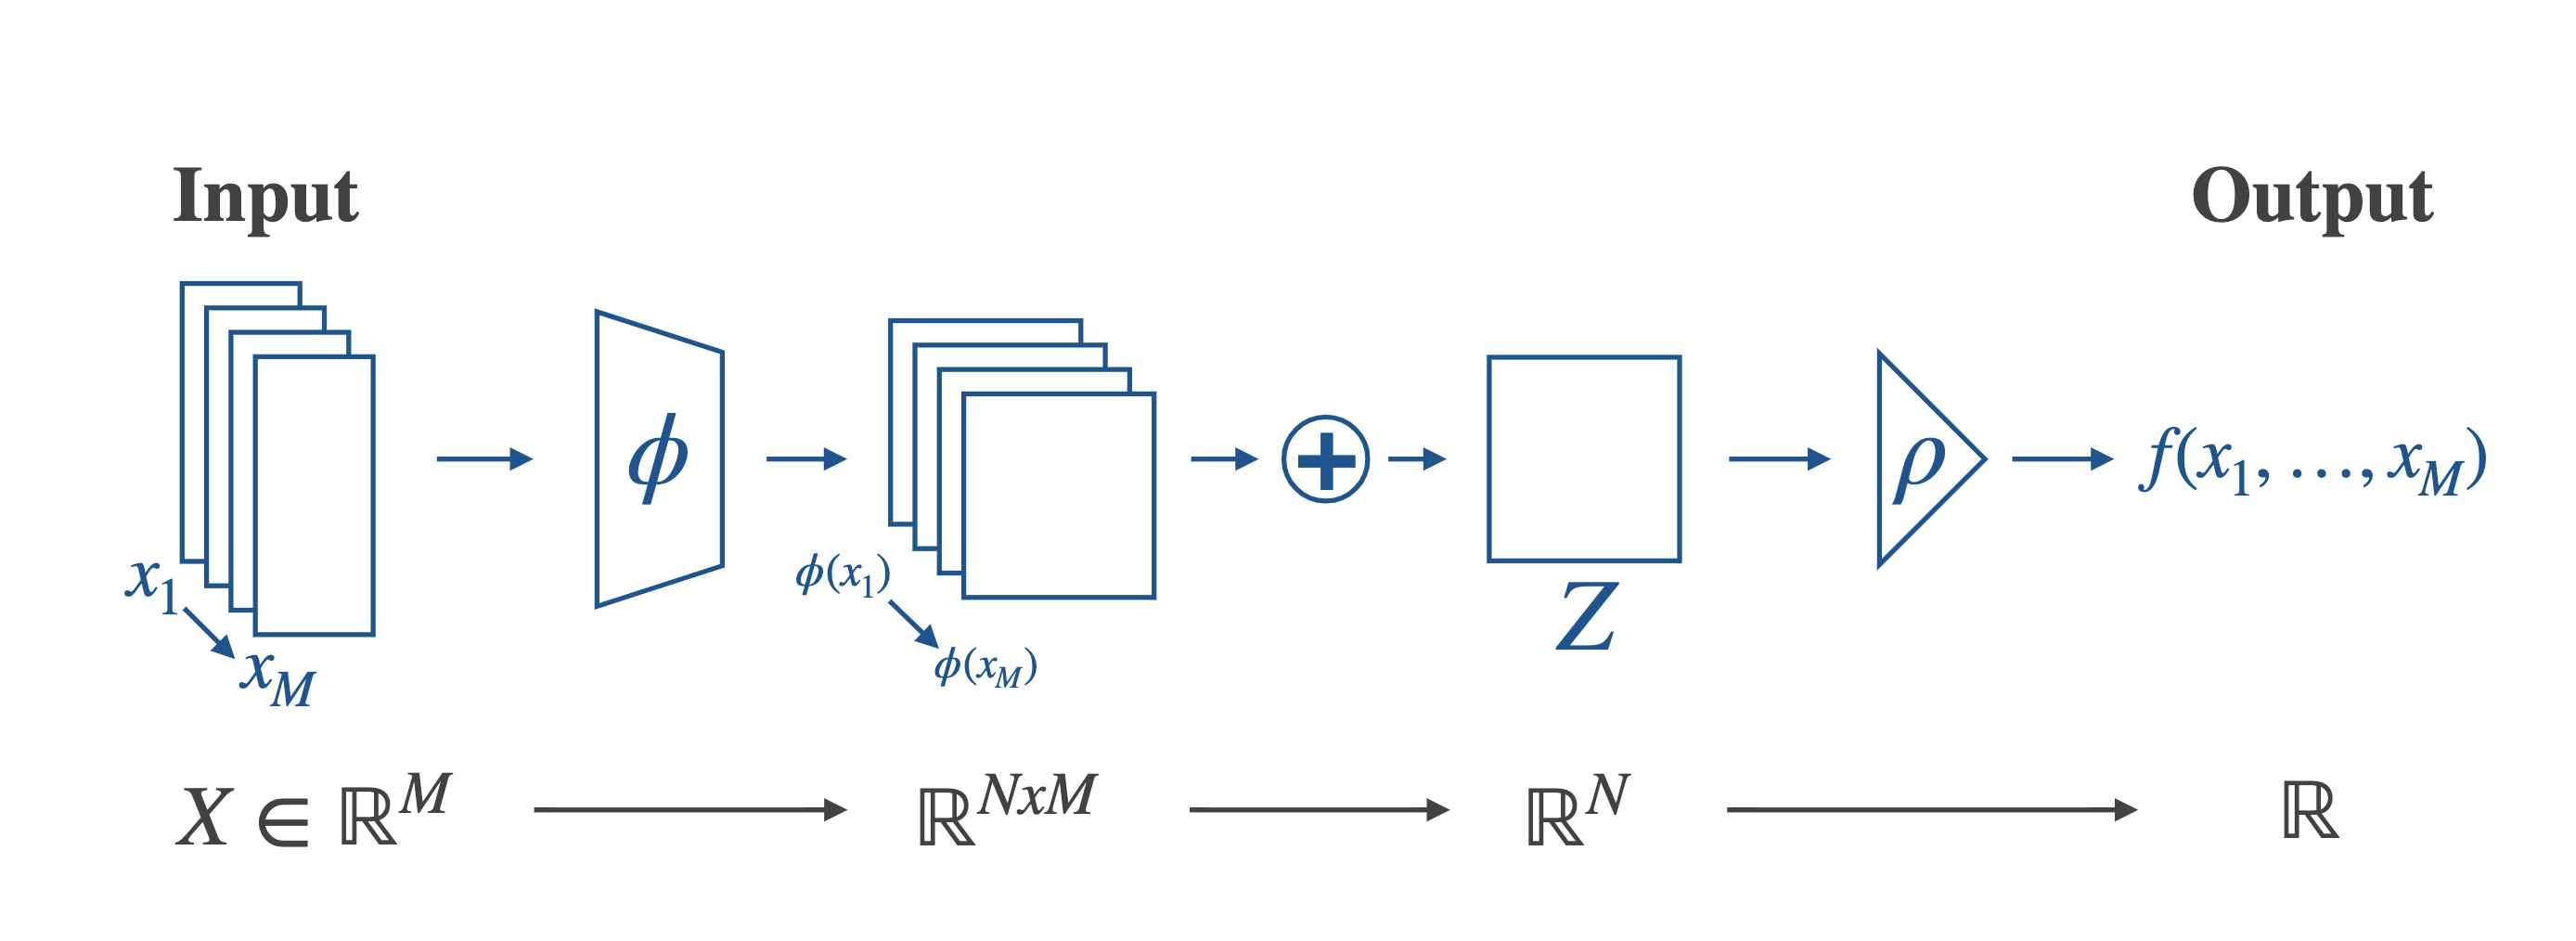
\includegraphics[width=\textwidth]{figures/deep-sets}
    \caption{Model structure of Deep Sets \citep{zaheer2017deep}.}
    \label{fig:deep-sets}
\end{figure}

Let $\phi: R \to \R^d$ be a pointwise feature extractor neural network, the Deep Sets architecture
\citep{zaheer2017deep} obtains an order-invariant representation of the input set by summing them
up, because the sum operation enforces order-invariant, \[
    \sum_{m=1}^{M} \phi(\vec{x}_m).
\]
We can then use this representation with any type of neural network $\rho: \R^d \to \mathcal{Y}$ to
get an order-invariant model, \[
    f(\vec{x}_1, \ldots, \vec{x}_M) = \rho \lft( \sum_{m=1}^{M} \phi(\vec{x}_m) \rgt).
\]
Once we have an order-invariant feature extractor, we can easily turn it into an equivariant map by
additionally providing $\vec{x}_m$ to $\rho: R \times \R^d \to \mathcal{Y}$ and applying $\rho$
pointwise, \[
    f(\vec{x}_1, \ldots, \vec{x}_M) = \lft( \rho \lft( \vec{x}_1, \sum_{m=1}^{M} \phi(\vec{x}_m) \rgt), \ldots, \rho \lft( \vec{x}_M, \sum_{m=1}^{M} \phi(\vec{x}_m) \rgt) \rgt).
\]
This architecture is universal for a fixed $d$, but it requires mappings that are highly
discontinuous as $M \to \infty$, which makes its usefulness limited in practice
\citep{wagstaff2019limitations}. More realistic mappings require $d \geq M$.

\subsection{PointNet}

\begin{figure}[t]
    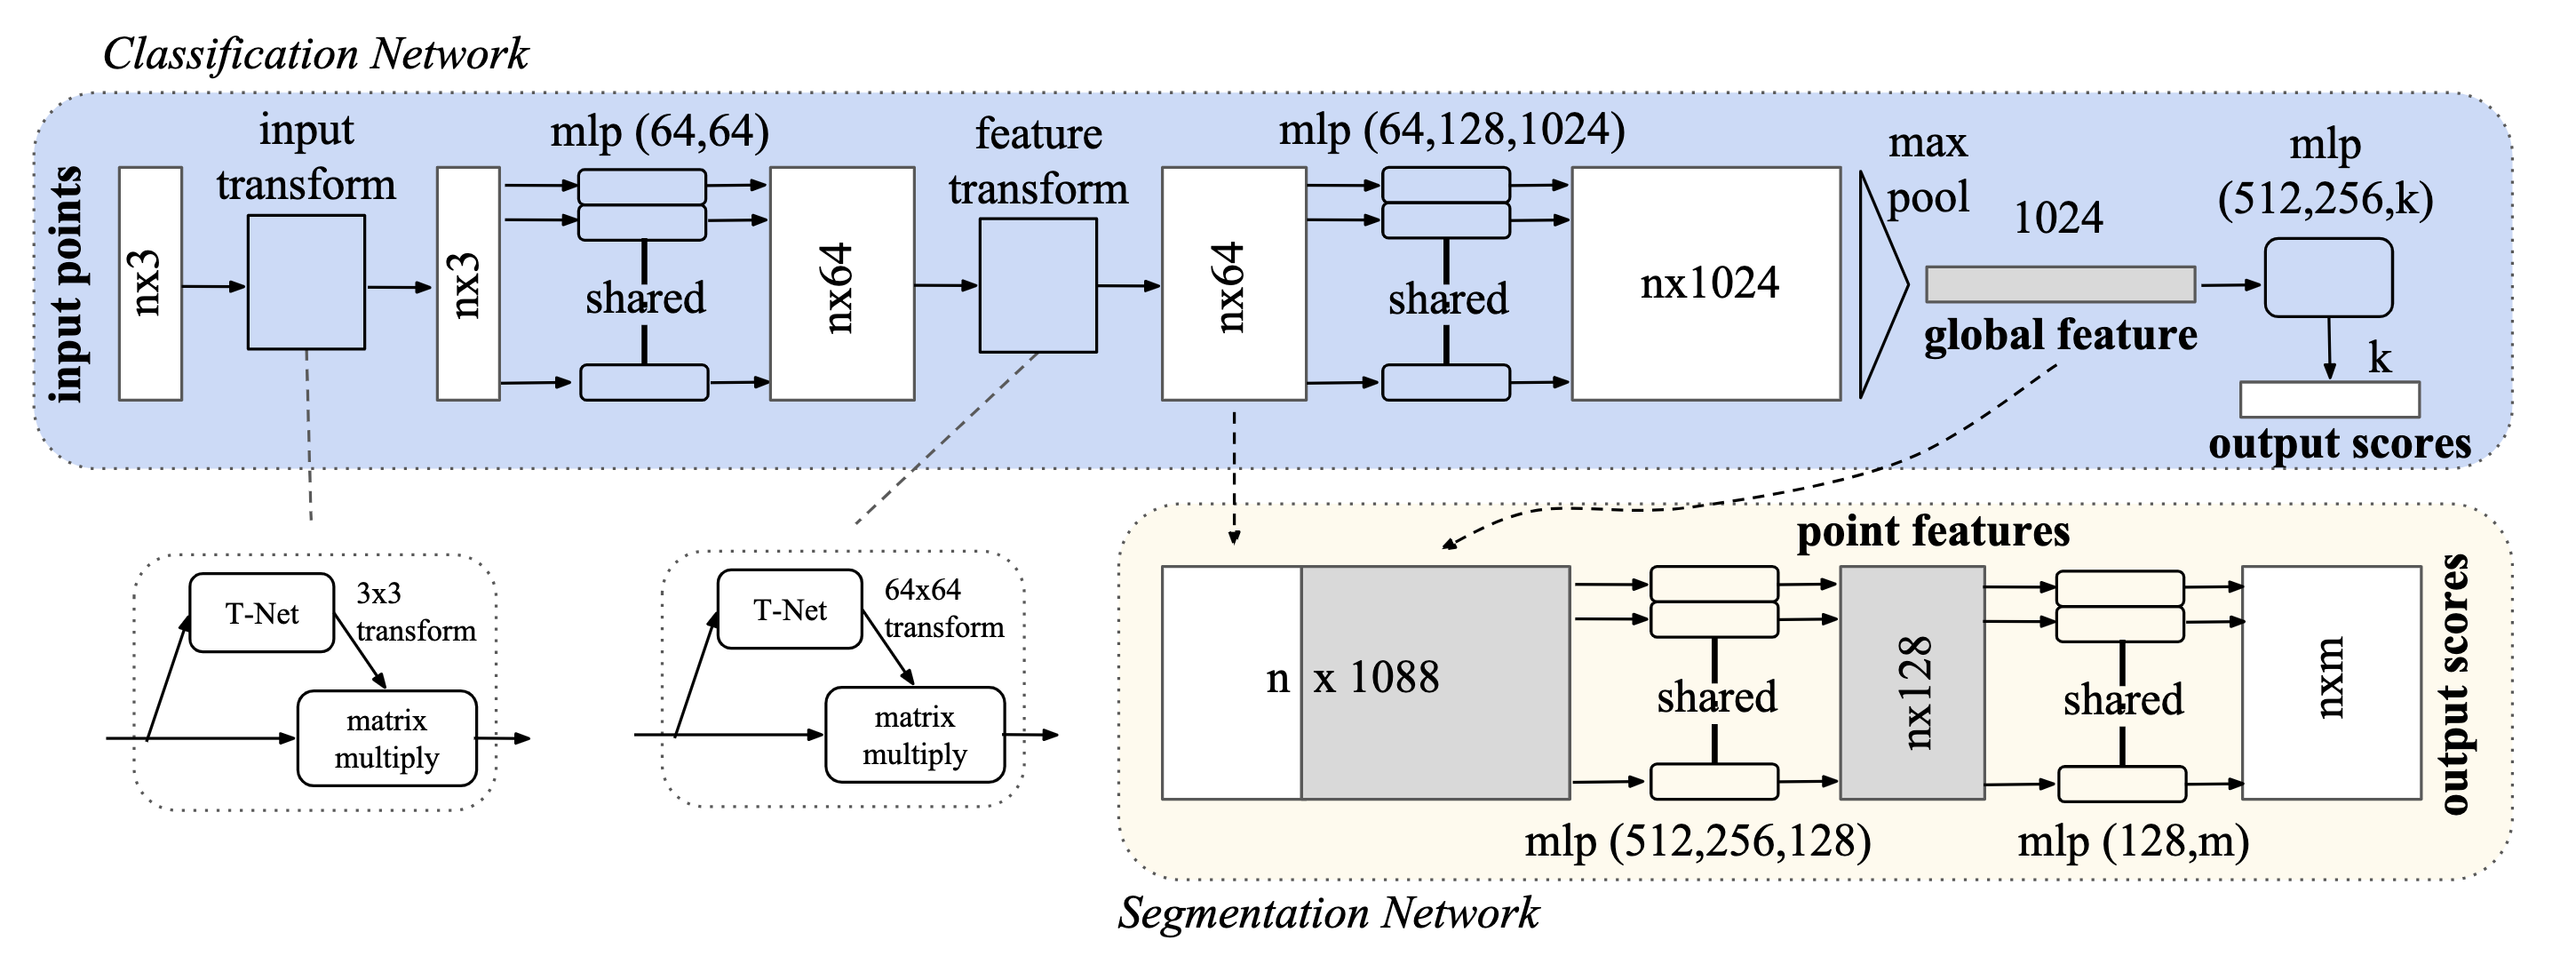
\includegraphics[width=\textwidth]{figures/pointnet}
    \caption{Model architecture of PointNet \citep{qi2017pointnet}.}
    \label{fig:pointnet}
\end{figure}

The PointNet model \citep{qi2017pointnet} is a specific use case of the Deep Sets architecture. The
model receives a set of three-dimensional points as input---a point cloud---and must classify the
object or segment its parts. The former use case requires an order-invariant model, while the
latter requires an equivariant model, because the order that the points are presented in does not
carry meaning.

This model employs T-net blocks, which apply rigid transformations to the input point cloud, which
is permutation invariant. These are applied alternatingly with multi-layer perceptrons to form a
permutation invariant feature extractor $\phi$. $\phi$ applies two stages of this, which result in
a $64$-dimensional intermediate feature vector and a $1024$-dimensional final feature vector. The
features are aggregated by a max-pool operator to obtain an order-invariant $1024$-dimensional
global feature vector.

For object classification, $\rho$ is implemented as a multi-layer perceptron with a softmax head
that takes the global feature vector as input. For object segmentation, $\rho$ concatenates the
intermediate local $64$-dimensional feature vector with the global $1024$-dimensional vector, which
is given to a multi-layer perceptron with a softmax head.

\subsection{Graph neural networks}

\begin{definition}[Graph]
    An undirected graph $G=(V, E)$ consists of vertices $V = \{ v_1, \ldots, v_M \}$ and edges $E = \{ e_1, \ldots, e_K \} \subseteq \{ \{ v, v' \} \mid v, v' \in V \}$.
\end{definition}

In GNNs (\textit{\textbf{G}raph \textbf{N}eural \textbf{N}etworks}), we associate a feature vector
$\vec{x}_m \in \R^d$ with each node $v_m \in V$. Let $\mat{X} \in \R^{M \times d}$ contain all
vertex feature vectors and $\mat{A} \in \R^{M \times M}$ be the adjacency matrix, where \[
    a_{ij} = \begin{cases}
        1 & \{ v_i, v_j \} \in E      \\
        0 & \{ v_i, v_j \} \not\in E.
    \end{cases}
\]

\begin{definition}
    A function $f$ on a graph with adjacency matrix $\mat{A}$ is order-invariant if and only if \[
        f(\mat{X}, \mat{A}) = f(\mat{P}\mat{X}, \mat{P}\mat{A}\transpose{\mat{P}}), \quad \mat{P} \in \Pi(M).
    \]
\end{definition}

\begin{definition}
    A function $f$ on a graph with adjacency matrix $\mat{A}$ is equivariant if and only if \[
        f(\mat{X}, \mat{A}) = \mat{P} f(\mat{P}\mat{X}, \mat{P}\mat{A}\transpose{\mat{P}}), \quad \mat{P} \in \Pi(M).
    \]
\end{definition}

We now want to design a model on graphs that is in- or equivariant. A common way to achieve this is
by parametrizing a local function that only depends on the neighbors of each vertex. Let $\mat{X}_m
    \doteq \{\!\{ \vec{x}_n \mid \{ v_n, v_m \} \in E \}\!\}$, which denotes the multiset of feature
vectors of the neighbors of $v_m$. We then parametrize a feature function $\phi$ that takes
$\vec{x}_m$ and $\mat{X}_m$ as input. (As a consequence, any pair of isomorphic graphs result in
the same feature representations.) This function must also be order-invariant to the neighbors, so
we need to additionally aggregate the neighbor feature vectors, which are processed by a separate
network $\psi$, \[
    \phi(\vec{x}_m, \mat{X}_m) = \phi \lft( \vec{x}_m, \bigoplus_{\vec{x}\in \mat{X}_m} \psi(\vec{x}) \rgt),
\]
where $\bigoplus$ is an invariant aggregation function. This is sometimes called a message-passing
scheme in the sense that a vertex receives messages from its neighbors via a messaging function
$\psi$ and uses an update function $\phi$ to update its representation.

\paragraph{Coupling matrix.}

In GCNs (\textit{\textbf{G}raph \textbf{C}onvolutional \textbf{N}etworks}), the aggregation over
local neighborhoods is performed with a fixed set of weights, known as the coupling matrix, \[
    \bar{\mat{A}} \doteq \mat{D}^{-\nicefrac{1}{2}} (\mat{A} + \mat{I}) \mat{D}^{-\nicefrac{1}{2}}, \quad \mat{D} = \mathrm{diag}(\vec{d}), d_m = 1 + \sum_{n=1}^{M} a_{nm}.
\]
Here, $\mat{D}$ is the degree matrix and $\bar{\mat{A}}$ is a normalized version of $\mat{A}$ with
self-loops as a result.

Furthermore, we introduce learnable parameters $\mat{W}$ that linearly transforms the vertex
feature vectors. Let $\sigma$ be an activation function, then the following is one step of
propagation in GCNs, \[
    \mat{\Xi} = \sigma(\bar{\mat{A}} \mat{X} \mat{W}), \quad \mat{W} \in \R^{d \times d'}.
\]
Note that $\bar{\mat{A}}$ operates on the node-edge structure and $\mat{W}$ operates in the feature
space. This layer can be stacked as in normal neural networks to introduce depth. A simple
two-layer GCN for node classification looks as follows, \[
    \mat{Y} = \mathrm{softmax}\lft( \bar{\mat{A}} \lft( \bar{\mat{A}} \mat{X} \mat{W}_0 \rgt)_+ \mat{W}_1 \rgt).
\]
As the depth increases, it is important to note that $\| \bar{\mat{A}} \|_2 \leq 1$, which ensures
that activations do not grow out out of control.

A limitation of GCNs is that it requires a depth equal to the diameter of the graph to exchange
information between all nodes. However, the problem with very deep GCNs is that feature vectors
between nodes become indistinguishable due to the smoothing that $\bar{\mat{A}}$ introduces
\citep{chen2020measuring}. Further, there is a bottleneck effect of how much information can be
stored in fixed-size representations \citep{alon2020bottleneck}. There are no general solutions to
these problems.

\paragraph{Attention.}

As we have already seen in transformers, the attention mechanism is permutation equivariant \wrt
the sequence order.\sidenote{This is due to the softmax operator being equivariant.} GATs
(\textit{\textbf{G}raph \textbf{A}ttention \textbf{N}etworks}) \citep{velivckovic2017graph} define
the coupling matrix $\mat{Q}$ using attention, \[
    q_{ij} = \mathrm{softmax}_j \lft( \rho \lft( \transpose{\vec{u}} [\mat{V} \vec{x}_i, \mat{V} \vec{x}_j, \vec{x}_{ij}] \rgt) \rgt),
\]
where $\mat{V}$ projects the node features and $\vec{x}_{ij}$ is a feature vector representing the
edge between $v_i$ and $v_j$. These are concatenated and projected to a learnable direction
$\vec{u}$. The advantage of this method is that the aggregation coefficients are now learnable,
instead of fixed equal weights.

Despite having a higher degree of adaptivity, a GAT is still a message-passing algorithm. Such
models have inherent limitations in the type of graphs that they can distinguish. The
Weisfeiler-Lehman graph isomorphism test computes whether there exists an isomorphism between two
graphs. \citet{morris2019weisfeiler} show that many message-passing algorithms---such as GCNs and
GATs---cannot distinguish graphs beyond the WL-test. Hence, there is a clear need for higher order
GNNs.

\subsection{Spectral graph theory}

\begin{definition}[Laplacian operator]
    The Laplacian is defined as \[
        \Delta f \doteq \sum_{i=1}^{d} \pdv[order=2]{f}{x_i}, \quad f: \R^d \to \R.
    \]
\end{definition}

Intuitively, the Laplacian measures the local deviation from the mean of $f$ in vanishingly small
neighborhoods.

\begin{definition}[Graph Laplacian]
    The graph Laplacian is defined as \[
        \mat{L} = \mat{D} - \mat{A},
    \]
    where $\mat{D}$ is the degree matrix and $\mat{A}$ is the adjacency matrix. Alternatively, the
    symmetric degree-normalized Laplacian can be used, \[
        \tilde{\mat{L}} = \mat{I} - \mat{D}^{-\nicefrac{1}{2}} \mat{A} \mat{D}^{-\nicefrac{1}{2}} = \mat{D}^{-\nicefrac{1}{2}} (\mat{D} - \mat{A}) \mat{D}^{-\nicefrac{1}{2}}.
    \]
\end{definition}

One can generalize the Fourier transform to graphs by making use of the diagonalization of the
Laplacian, \[
    \mat{L} = \mat{U} \mat{\Lambda} \transpose{\mat{U}}.
\]
The columns of the orthogonal matrix $\mat{U}$ can be seen as the graph Fourier basis and the
eigenvalues as frequencies. The convolution can then be defined as pointwise multiplication in the
Fourier domain, \[
    \vec{x} * \vec{y} = \mat{U} (\transpose{\mat{U}} \vec{x} \odot \transpose{\mat{U} \vec{y}}).
\]
The learned convolution operation from one-dimensional signals is generalized as follows, \[
    G_{\vec{\theta}}(\mat{L})\vec{x} = \mat{U}G_{\vec{\theta}}(\mat{\Lambda}) \transpose{\mat{U}}\vec{x}.
\]
The problem with this approach is that computing the eigendecomposition of $\mat{L}$ is done in
$\bigo{M^3}$. A trick to circumvent this problem is to use polynomial kernels, \[
    \mat{U} \lft( \sum_{k=0}^{K} \alpha_k \mat{\Lambda}^k \rgt) \transpose{\mat{U}} = \sum_{k=0}^{K} \alpha_k \mat{L}^k.
\]
Here, the polynomial order $K$ defines the size of the neighborhood, \ie, the kernel size. The
parameters of this model are $\alpha_k$, so the number of parameters---and hence the
expressivity---of this layer is much smaller than in traditional one-, two-, or three-dimensional
convolutions.

Motivated by spectral graph theory, we can define a graph-convolutional layer as \[
    \vec{\xi}_m = \sum_{n=1}^{M} p_{mn}(\mat{L}) \vec{x}_n + b_n, \quad p_{mn}(\mat{L}) \doteq \sum_{k=0}^{K} \alpha_{mnk} \mat{L}^k.
\]
As before, $K$ defines the ``kernel size'' and $\vec{\alpha}$ are the parameters, which is used to
compute the coefficients of the neighbors. As in traditional convolutions, this can be expressed as
an affine transformation.
